\documentclass[11pt, oneside]{article}   	% use "amsart" instead of "article" for AMSLaTeX format
\usepackage{geometry}                		% See geometry.pdf to learn the layout options. There are lots.
\geometry{letterpaper}                   		% ... or a4paper or a5paper or ... 
%\geometry{landscape}                		% Activate for for rotated page geometry
%\usepackage[parfill]{parskip}    		% Activate to begin paragraphs with an empty line rather than an indent
\usepackage{graphicx}				% Use pdf, png, jpg, or eps� with pdflatex; use eps in DVI mode
								% TeX will automatically convert eps --> pdf in pdflatex		
\usepackage{amssymb}
\graphicspath{{/Users/telliott_admin/Dropbox/Tex/png/}}

\title{Law of Cosines}
%\author{The Author}
\date{}							% Activate to display a given date or no date

\begin{document}
\maketitle
%\section{}
%\subsection{}
\setlength{\parskip}{2 mm}
\large
In this short write-up, we'll work through an algebraic proof of the law of cosines.  In the triangle below, $A$, $B$, and $C$ are the angles, with side lengths $a$, $b$, and $c$.

\begin{center}
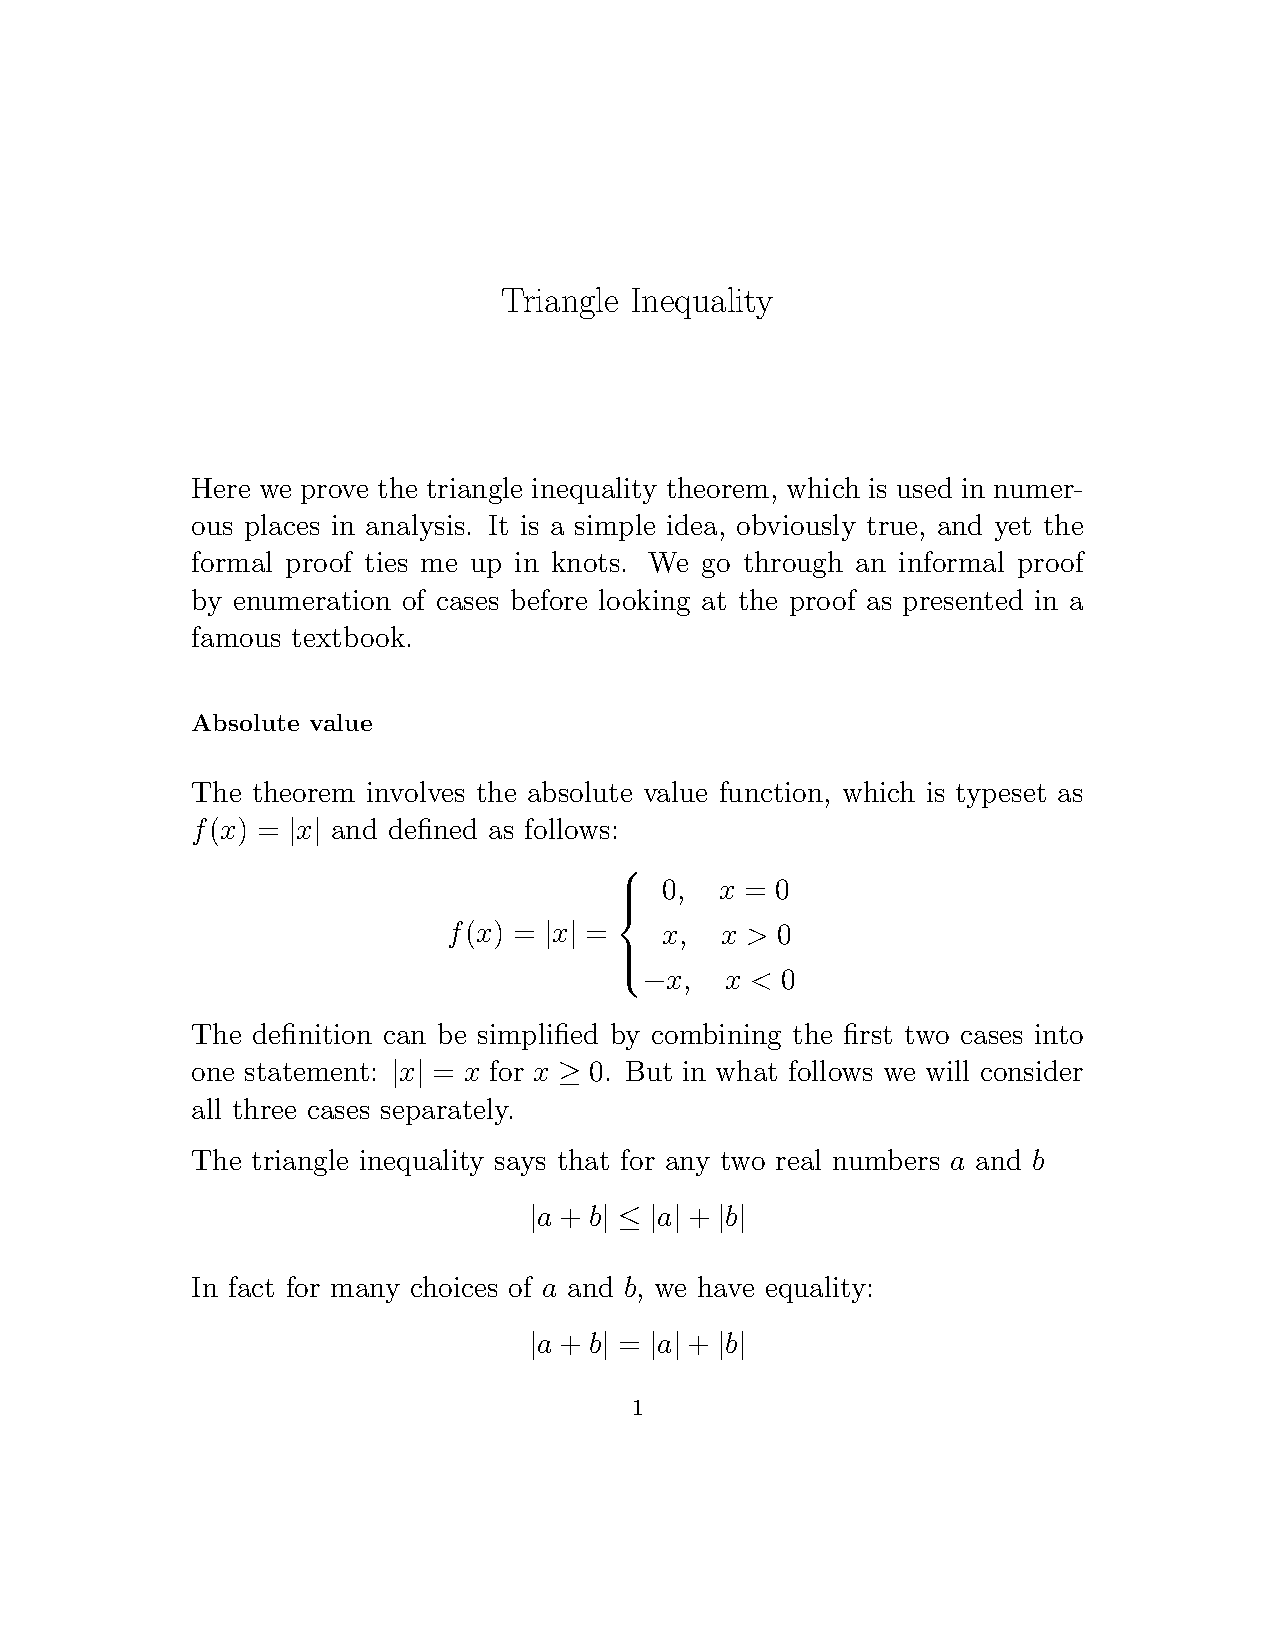
\includegraphics [scale=0.5] {triangle.png}
\end{center}

An altitude has been drawn from angle $C$ to side $c$ opposite.  The altitude is perpendicular to the side $c$, which is thereby divided into lengths $d$ and $e$.

We'll use these four facts
\[ c = d + e \]
\[ a^2 = e^2 + h^2 \] 
\[ b^2 = d^2 + h^2 \] 
\[  \frac{d}{b} = \cos A \]

Start with

\[ a^2 = e^2 + h^2 \] 

Knowing that

\[ b^2 = d^2 + h^2 \]
\[ h^2 = b^2 - d^2 \]

substitute for $h^2$

\[ a^2 = e^2 + b^2 - d^2 \]

Since $e = c - d$, substitute for $e^2$

\[ a^2 = (c-d)^2 + b^2 - d^2 \]
\[  = c^2 -2cd + d^2 + b^2 - d^2 \]
\[  = b^2 + c^2 -2cd \]

Finally, substitute for $d$ knowing that $d= b \cos A$

\[  a^2 = b^2 + c^2 -2bc \cos A \]
QED.

This is the Law of Cosines.

Notice that if $A = 90^\circ$, $d=0$ and $cos A = 0$, and this becomes the Pythagorean Theorem.

Another way, which is slightly shorter:

\begin{center}
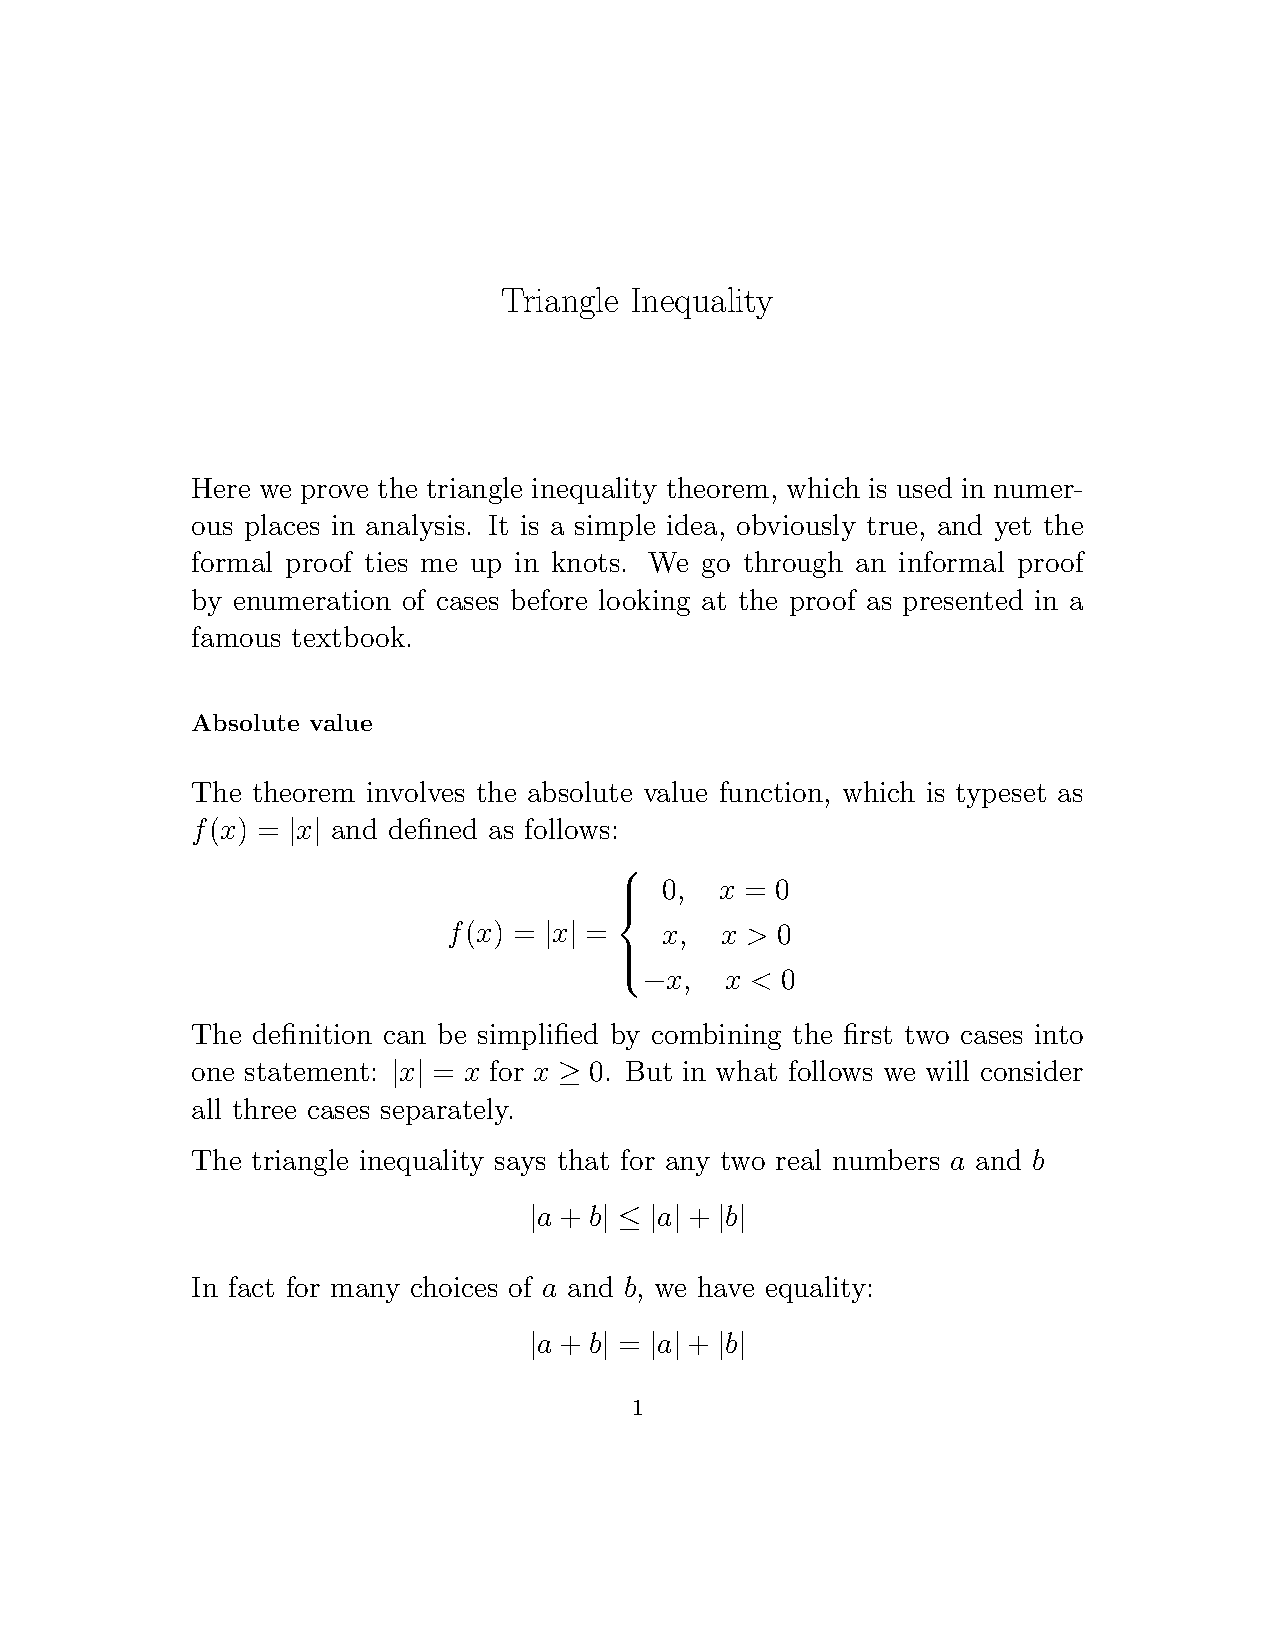
\includegraphics [scale=0.5] {triangle.png}
\end{center}

\[ d = b \cos A \]
\[ e = c - d = c - b \cos A \]
\[ h = b \sin A \]

So, using Pythagoras

\[ a^2 = h^2 + e^2 \]
\[ = b^2 \sin^2 A + c^2 - 2 bc \cos A + b^2 \cos^2 A \]
\[ = b^2 + c^2 - 2bc \cos A \]


\end{document}  